\documentclass[tikz,border=8pt]{standalone}
\usepackage[T1]{fontenc}
\usepackage{lmodern}
\renewcommand{\familydefault}{\sfdefault}
\usetikzlibrary{positioning,arrows.meta,calc}

\tikzset{
  box/.style={draw, rounded corners=2pt, align=center, font=\small\sffamily,
    fill=white, inner sep=4pt, minimum height=9mm, text width=62mm},
  gate/.style={box, fill=black!3, text width=66mm, align=left, font=\footnotesize\sffamily},
  arrow/.style={-{Latex[length=2mm,width=1.3mm]}, semithick},
  lbl/.style={font=\scriptsize\sffamily, fill=white, inner sep=1pt, align=center}
}

\begin{document}
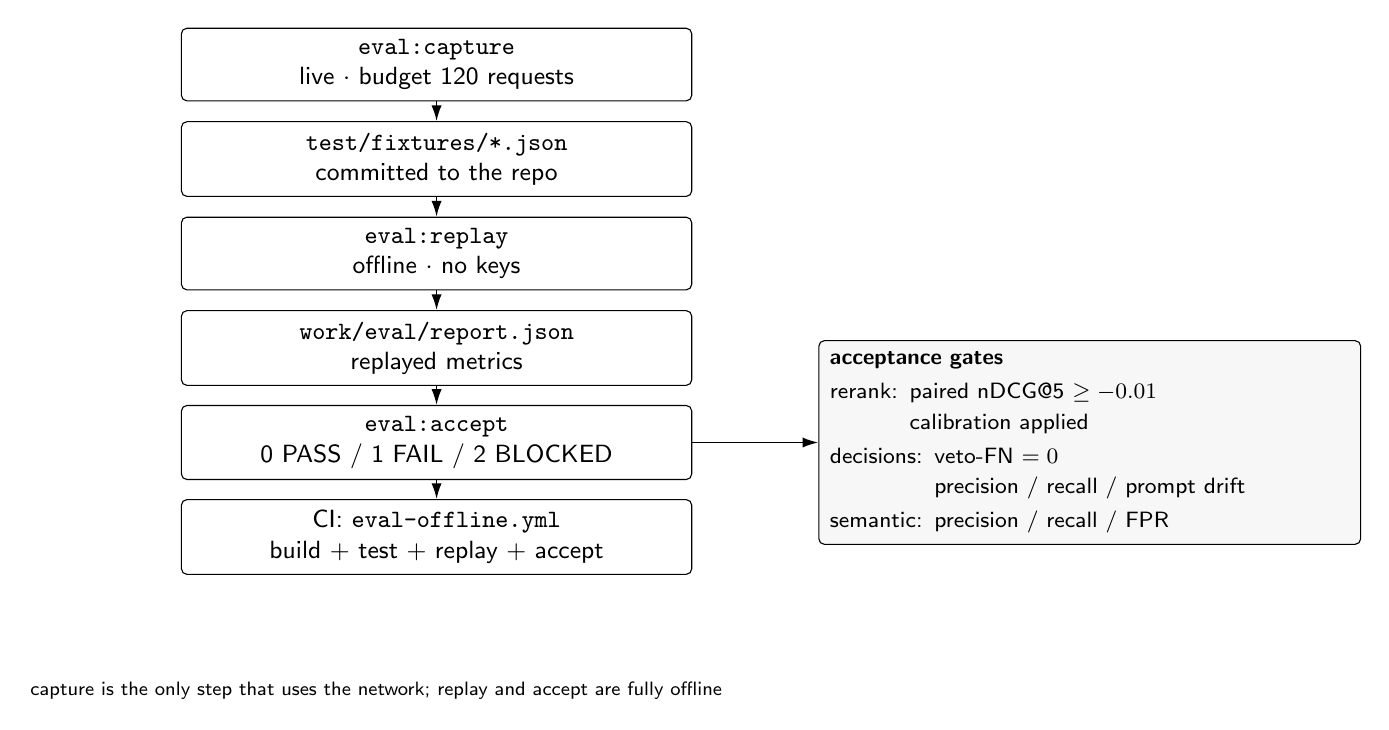
\begin{tikzpicture}

\node[box] (cap) at (0,6.2) {\texttt{eval:capture}\\live $\cdot$ budget 120 requests};
\node[box] (fix) at (0,5.0) {\texttt{test/fixtures/*.json}\\committed to the repo};
\node[box] (rep) at (0,3.8) {\texttt{eval:replay}\\offline $\cdot$ no keys};
\node[box] (rpt) at (0,2.6) {\texttt{work/eval/report.json}\\replayed metrics};
\node[box] (acc) at (0,1.4) {\texttt{eval:accept}\\0 PASS / 1 FAIL / 2 BLOCKED};
\node[box] (ci) at (0,0.2) {CI: \texttt{eval-offline.yml}\\build + test + replay + accept};

\draw[arrow] (cap) -- (fix);
\draw[arrow] (fix) -- (rep);
\draw[arrow] (rep) -- (rpt);
\draw[arrow] (rpt) -- (acc);
\draw[arrow] (acc) -- (ci);

\node[gate, right=16mm of acc] (gates)
  {\textbf{acceptance gates}\\[1mm]
   rerank: paired nDCG@5 $\ge -0.01$\\[0.5mm]
   \phantom{rerank: }calibration applied\\[1mm]
   decisions: veto-FN $=0$\\[0.5mm]
   \phantom{decisions: }precision / recall / prompt drift\\[1mm]
   semantic: precision / recall / FPR};
\draw[arrow] (acc.east) -- (gates.west);

\node[lbl, anchor=north west, fill=none] at (-5.2,-1.6)
  {capture is the only step that uses the network; replay and accept are fully offline};

\end{tikzpicture}
\end{document}
